\documentclass{amsart}
\usepackage[utf8]{inputenc}

\usepackage{fullpage}

%! TeX root = ./main.tex

\usepackage{xifthen}

\usepackage{amsmath}

\DeclareMathOperator{\I}{i}
\DeclareMathOperator{\DOp}{d}
\DeclareMathOperator*{\Argmin}{argmin}

\usepackage{amssymb}
\usepackage{bm}
\usepackage{upgreek}
\usepackage{mathrsfs}

\newcommand{\Abs}[1]{\lvert#1\rvert}
\newcommand{\BigAbs}[1]{\left\lvert#1\right\rvert}

\renewcommand{\Vec}[1]{\bm{#1}}
\newcommand{\Grad}[1][]{\bm{\nabla}#1}
\newcommand{\Laplacian}[1][]{\Delta#1}
\newcommand{\Norm}[2][]{\lVert#2\rVert\ifthenelse{\isempty{#1}}{}{_{#1}}}
\newcommand{\BigNorm}[2][]{\left\lVert#2\right\rVert\ifthenelse{\isempty{#1}}{}{_{#1}}}
\newcommand{\InProd}[3][]{\langle#2,#3\rangle\ifthenelse{\isempty{#1}}{}{_{#1}}}
\newcommand{\BigInProd}[3][]{\left\langle#2,#3\right\rangle\ifthenelse{\isempty{#1}}{}{_{#1}}}

\newcommand{\Card}[1]{\lvert#1\rvert}
\newcommand{\Ord}{\mathcal{O}}

\newcommand{\D}{\DOp\!}

\newcommand{\CE}{\mathcal{E}}
\newcommand{\CH}{\mathcal{H}}
\newcommand{\CV}{\mathcal{V}}

\newcommand{\SL}{\mathscr{L}}

\newcommand{\DN}{\mathbb{N}}
\newcommand{\DZ}{\mathbb{Z}}
\newcommand{\DR}{\mathbb{R}}
\newcommand{\DC}{\mathbb{C}}

\usepackage{amsthm}

\newtheorem{proposition}{Proposition}

\usepackage{graphicx}
\usepackage{subcaption}
\usepackage{tikz}

\usetikzlibrary{automata}


\title{Fast Solvers for Quantum Rotors}

\begin{document}

\maketitle

\section{Introduction}

\subsection{Problem Statement}

Let $(\CV, \CE)$ be an undirected graph with vertex set $\CV = \{1, \ldots,
d\}$ for some $d \geq 2$ and edge set $\CE \subseteq \{(j, k) \in \CV \times
\CV : j \neq k\}$ (i.e.\ we don't consider graphs with self-loops). We can
envision a system of quantum rotors on this graph, where the vertices
correspond to the rotors, and the edges define some interaction between the
rotors. The Hamiltonian of such a system may be written as
\begin{equation}
  H = - \frac{1}{2} \Laplacian - \sum_{(j, k) \in \CE} g_{jk} \cos(\theta_j -
  \theta_k)
\end{equation}
Our goal is to find a solution of the associated Schrodinger equation
\begin{equation}
  \label{eq:schrodinger}
  H \psi(\Vec{x}) = \lambda \psi(\Vec{x})
\end{equation}
that has the minimum energy. We shall restrict ourselves to only the
wavefunctions $\psi \in \SL^1([0, 2\pi]^d)$ and their weak derivatives satisfy
periodic boundary conditions.

\subsection{Reformulation Using Fourier Series}

Since $\psi$ is $2\pi$-periodic along each of the dimensions, we can express it
in terms of the Fourier series
\begin{equation}
  \label{eq:fourier}
  \psi(\Vec{x}) = \frac{1}{(2 \pi)^d} \sum_{\Vec{\omega} \in \DZ^d}
  \hat{\psi}(\Vec{\omega}) \exp(\I \Vec{\omega} \cdot \Vec{\theta})
\end{equation}
where ``$\,\cdot\,$'' is the standard inner product in $\DR^d$ and the Fourier
coefficients are given by
\begin{equation}
  \hat{\psi}(\Vec{\omega}) := \int_{[0, 2\pi]^d} \psi(\Vec{\theta}) \exp(-\I
  \Vec{\omega} \cdot \Vec{\theta}) \D{\Vec{\theta}}
\end{equation}
Now, substituting \eqref{eq:fourier} in \eqref{eq:schrodinger}, multiplying by
$\exp(\I \Vec{\omega} \cdot \Vec{\theta})$ and integrating over all space, we
obtain
\begin{equation}
  \label{eq:fourier-eigenstate}
  \Norm{\Vec{\omega}}^2 \hat{\psi}(\Vec{\omega}) - \frac{1}{2} \sum_{(j, k) \in
  \CE} g_{jk} [\hat{\psi}(\Vec{\omega} + \Vec{e}_j - \Vec{e}_k) +
  \hat{\psi}(\Vec{\omega} - \Vec{e}_j + \Vec{e}_k)] = \lambda
  \hat{\psi}(\Vec{\omega})
\end{equation}
where $\Vec{e}_j$ is the vector of all zeros except at the $j$-th entry, which
is $1$. Clearly, \eqref{eq:fourier-eigenstate} is an eigenvalue equation for
the Fourier coefficients $\hat{\psi}$ w.r.t.\ the operator $\hat{H}$ defined as
\begin{equation}
  \hat{H} \hat{\psi}(\Vec{\omega}) := \Norm{\Vec{\omega}}^2
  \hat{\psi}(\Vec{\omega}) - \frac{1}{2} \sum_{(j, k) \in \CE} g_{jk}
  [\hat{\psi}(\Vec{\omega} + \Vec{e}_j - \Vec{e}_k) + \hat{\psi}(\Vec{\omega} -
  \Vec{e}_j + \Vec{e}_k)]
\end{equation}
Note that given $\psi \in \SL^1([0, 2\pi]^d)$ with peridic weak derivatives,
the Fourier coefficients $\hat{\psi} \in \SL^2(\DZ^d)$ satisfy a fast decay
condition
\begin{equation}
  \sum_{\Vec{\omega} \in \DZ^d} \Norm{\Vec{\omega}}^2
  \Abs{\hat{\psi}(\Vec{\omega})} < \infty
\end{equation}

\section{Overview of Algorithms for Finding Extremal Eigenpairs}

\subsection{Problem Statement}

In a separable Hilbert space $\CH$, let $A : \CH \to \CH$ be non-zero, positive
semi-definite, compact, Hermitian. We want to find it is maximal eigenpair. The
existence of the maximal eigenpair for $A$ follows from the spectral theorem.

\subsection{Connection to Our Problem}

In our problem, we can easily establish a lower bound for the minimal eigevalue
of our Hamiltonian $H$; it is given by
\begin{equation}
  \lambda_\text{min}(H) \geq \mu = -\sum_{(j, k) \in \CE} \Abs{g_{jk}}
\end{equation}
It turns out that the operator $A = (H - \mu I)^{-1}$ is non-zero, positive
semi-definite, compact (?) and Hermitian. Additionally, our space of functions
$\SL^1([0, 2\pi]^d)$ is a Hilbert space and is separable with the Fourier basis
\begin{equation}
  \left\{e^{\I \Vec{\omega} \cdot \Vec{\theta}} : \Vec{\omega} \in \DZ^d\right\}
\end{equation}
Thus, we can find the maximal eigenpair of the operator $A$, which corresponds
to the minimal eigenpair of the Hamiltonian $H$.

\subsection{Power Iteration}

Given an arbitrary state $\psi_0$, consider the sequence $\psi_\ell$ and
\begin{equation}
  \psi_{\ell + 1} = \frac{A \psi_\ell}{\Norm[\CH]{A \psi_\ell}}, \quad
  \lambda_{\ell + 1} = \InProd[\CH]{\psi_{\ell + 1}}{A \psi_{\ell + 1}}
\end{equation}
Now provided
\begin{enumerate}
  \item
    The maximal eigenpair is unique
  \item
    Initial state $\psi_0$ is not orthogonal to the eigenstate of the maximal
    eigenpair
\end{enumerate}
the power iteration converges to the maximal eigenpair. When we apply this
approach to $A = (H - \mu I)^{-1}$ to find the minimal eigenpair of $H$, this
algorithm is called the inverse power iteration.

\subsection{Rayleigh Quotient Iteration}

Rayleigh quotient iteration improves the convergence of the inverse power
iteration by updating the $\mu$ value at each iteration: starting from $\mu_0 =
\mu$ we generate the next states as
\begin{equation}
  \psi_{\ell + 1} = \frac{(H - \mu_\ell I)^{-1} \psi_\ell}{\Norm[\CH]{(H -
  \mu_\ell I)^{-1} \psi_\ell}}, \quad \mu_{\ell + 1} =
  \frac{\InProd[\CH]{\psi_{\ell + 1}}{H \psi_{\ell +
  1}}}{\InProd[\CH]{\psi_{\ell + 1}}{\psi_{\ell + 1}}}
\end{equation}

\subsection{Projected Gradient Descent}

Finding the smallest eigenpair of $H$ can also be found by minimizing the
Rayleigh quotient. This is equivalent to solving the optimization problem
\begin{equation}
  \text{minimize} \quad \InProd[\CH]{\psi}{H \psi} \quad \text{subject to}
  \quad \Norm[\CH]{\psi} = 1
\end{equation}

\section{Numerical Solution Schemes}

All the algorithms outlined in the section above only require either applying
shifted Hamiltonian inverse $(H - \mu I)^{-1}\psi$ (i.e.\ solving the linear
system $(H - \mu I) \tilde{\psi} = \psi$) or computing the operator application
$H \psi$. Now, we outline a few different ways to actually implement this
operator application numerically.

\subsection{Finite Difference Scheme}

We discretize the quantum state $\psi$ on a uniform grid in the domain $[0,
2\pi]^d$ with $n$ points per dimension (technically, $n + 1$ points per
dimension, but the first and last points are the same due to periodicity). This
creates a $d$-dimensional $n \times \cdots \times n$ tensor discretization of
the state---we denote it as $\uppsi$.

Evaluating the discretization of $H \psi$ is straightforward provided we use
some finite difference scheme for the derivatives. For instance, we can use the
five-point finite difference stencil to approximate
\begin{equation}
  \frac{\partial^2 \psi}{\partial \theta_j^2}(\Vec{i} h) \approx
  \frac{-\uppsi(\Vec{i}_j^{(+2)}) + 16 \uppsi(\Vec{i}_j^{(+1)}) - 30
  \uppsi(\Vec{i}) + 16 \uppsi(\Vec{i}_j^{(-1)}) - \uppsi(\Vec{i}_j^{(-2)})}{12
  h^2}
\end{equation}
where we denote $\Vec{i} h = (i_1 h, \ldots, i_d h)$, $\Vec{i} = (i_1, \ldots,
i_d)$, and
\begin{equation}
  \Vec{i}_j^{(\pm k)} = (i_1, \ldots, i_{j - 1}, i_j^{(\pm k)}, i_{j + 1},
  \ldots, i_d), \quad i_j^{(\pm k)} = (i_j \pm k) \mod (n)
\end{equation}
with $0 \leq i_j < n$, $h = 2 \pi / n$. With this, we can now compute a
discretization of $(H - \mu I) \psi$ with fourth order accuracy very easily,
which in turn allows us to solve the system
\begin{equation}
  (H - \mu I) \widetilde{\psi}_{\ell + 1} = \psi_{\ell}
\end{equation}
using, for example, the conjugate gradient (CG) iterative method.

\subsection{Fourier Spectral Scheme}

Here we consider the Fourier reformulation of our problem. It is easy to see
that if $\hat{\psi}$ is a real-valued function, then so is $\hat{H}
\hat{\psi}$. To take advantage of this property, we start with the initial
state
\begin{equation}
  \psi^{(0)}(\theta_1, \ldots, \theta_d) = \cos(\theta_1) \cdots \cos(\theta_d)
\end{equation}
The corresponding Fourier coefficients are given by
\begin{equation}
  \hat{\psi}^{(0)}(k_1, \ldots, k_d) =
  \begin{cases}
    \pi^d & \text{if} \quad \Abs{k_1} = \cdots = \Abs{k_d} = 1 \\
    0 & \text{otherwise}
  \end{cases}
\end{equation}
Now due to the fast decay condition of the Fourier coefficients $\hat{\psi}$,
we can choose to compute $\hat{\psi}$ at the integer lattice points inside
$[-k_\text{max}, k_\text{max}]^d$ and assume the Fourier coefficients to be
zero outside this domain, without incurring too much error. We can now easily
evaluate $\hat{H} \hat{\psi}$, and consequently solve the linear system
$(\hat{H} - \mu \hat{I}) \hat{\phi} = \hat{\psi}_\ell$ using iterative methods.
To accelerate convergence of these iterative solvers, we devise a
preconditioner
\begin{equation}
  \hat{M} \hat{\psi}(\Vec{\omega}) = \left(\frac{1}{2} \Norm{\Vec{\omega}}^2 -
  \mu\right)^{1/2} \hat{\psi}(\Vec{\omega})
\end{equation}
and solve the preconditioned linear system
\begin{equation}
  \hat{M}^{-1} \Hat{H} \Hat{M}^{-1} \hat{M} \hat{\phi} = \hat{M}^{-1}
  \hat{\psi}
\end{equation}
Note that due to the symmetric nature of the preconditioning, we can still use
the iterative CG solver.

\section{Numerical Results}

\subsection{Self-Convergence of the Basic Scheme}

\begin{figure}
  \centering
  \begin{subfigure}{0.48\textwidth}
    \centering
    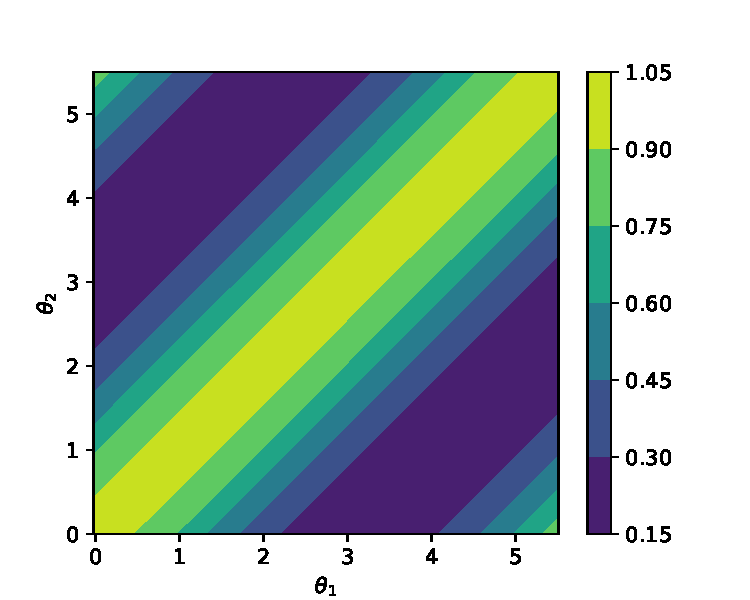
\includegraphics[width=\textwidth]{figures/2d_basic_self_convergence_state_1.pdf}
    \caption{$n = 8$}
  \end{subfigure}
  ~
  \begin{subfigure}{0.48\textwidth}
    \centering
    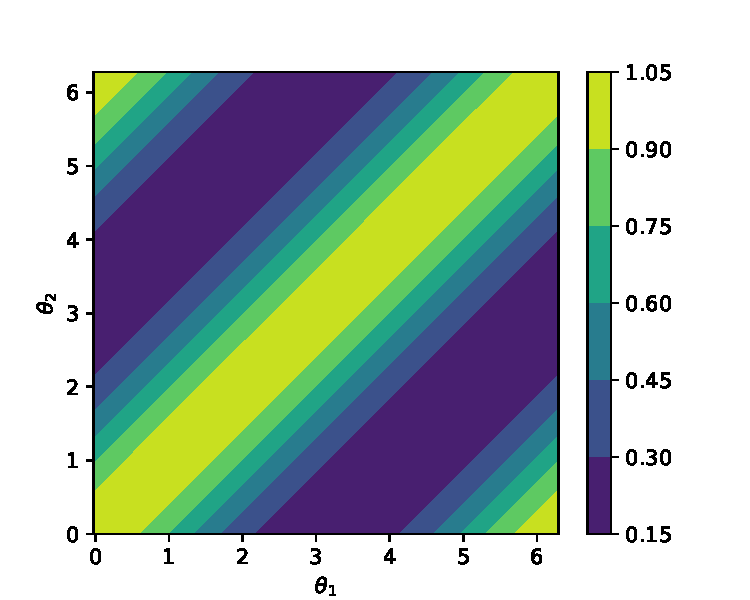
\includegraphics[width=\textwidth]{figures/2d_basic_self_convergence_state_8.pdf}
    \caption{$n = 1024$}
  \end{subfigure}
  \caption{The computed eigenstate corresponding to minimal energy at different
  number of grid points using the basic scheme. By visual inspection, these two
  solutions seem fairly close.}
  \label{fig:2d-basic-self-convergence-solution}
\end{figure}

\begin{figure}
  \centering
  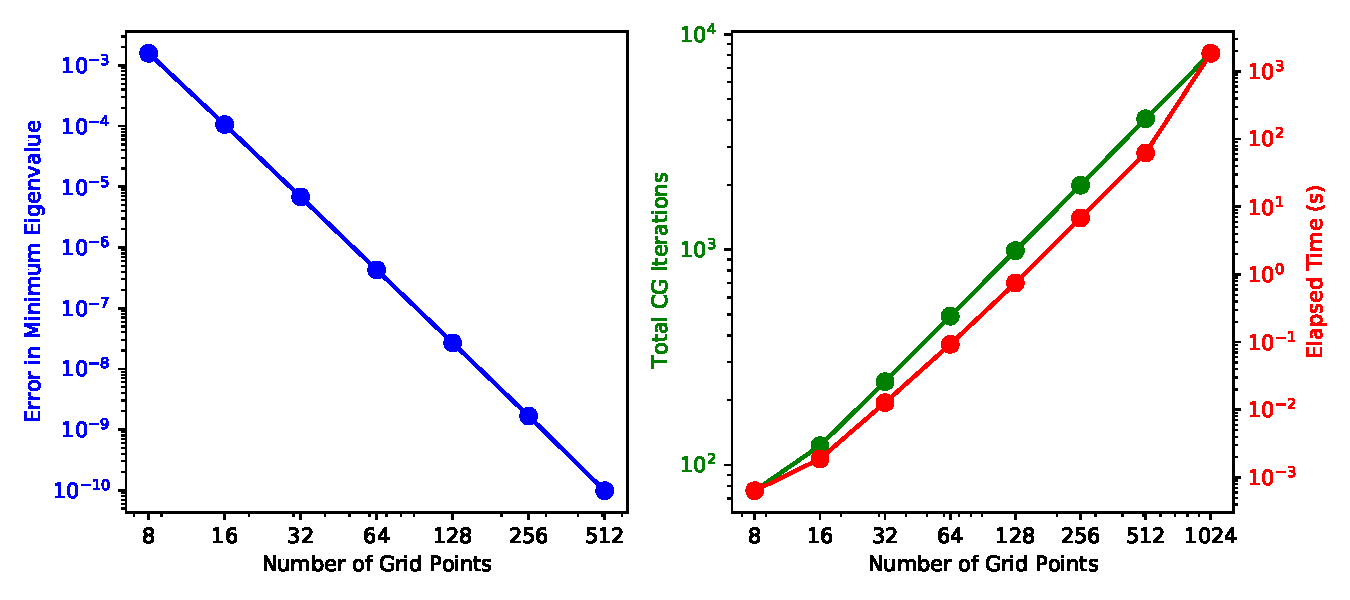
\includegraphics[width=\textwidth]{figures/2d_basic_self_convergence_analysis.pdf}
  \caption{\textbf{Left:} Error in minimal eigenvalue estimate, computed using
  the basic scheme, with increasing number of grid points $n$ per dimension.
  The $n = 1024$ grid point solution is used as the reference. The error of
  eigenvalue estimate decreases approximately as $\Ord(n^{-3.990829})$, which
  is consistent with our fourth-order derivative scheme. \textbf{Right} Total
  number of CG iterations, and the computing time, needed to construct the
  lowest energy eigenstate estimate with increasing number of grid points $n$
  using the basic scheme. Number of iterations increase approximately as
  $\Ord(n^{0.982632})$, and elapsed time increase approximately as
  $\Ord(n^{3.125835})$.}
  \label{fig:2d-basic-self-convergence-analysis}
\end{figure}

We performed a self-convergence analysis with this basic scheme in $d = 2$
dimensions with edge set $\CE = \{(1, 2)\}$ and $n = 8, 16, 32, \ldots, 1024$
uniform discretization points per dimension. We started our power iteration
with initial state
\begin{equation}
  \psi^{(0)}(\theta_1, \theta_2) = \cos(\theta_1) \cos(\theta_2)
\end{equation}
which is the lowest energy eigenstate corresponding to the Laplacian part of
the Hamiltonian. We set both the CG iteration and inverse power iteration
tolerances to $\tau_\text{cg} = \tau_\text{inv} = 10^{-6}$ --- the power
iteration is stopped when we get $\Abs{\lambda^{(\ell + 1)} - \lambda^{(\ell)}}
< \tau_\text{inv}$. In our example, it took 9 power iterations until
convergence to the minimal eigenstate at all discretization levels. Using the
$n = 1024$ discretization solution as the reference the lowest energy turns out
to be $\lambda_\text{min} \approx -0.378$. In
Figure~\ref{fig:2d-basic-self-convergence-analysis} we plot the errors of the
other discretization levels using this reference solution. The error decays
approximately as $\Ord(n^{-3.990829})$ as we increase the level of
discretization with our fourth order differentiation scheme. In the same
figure, we see that the number of total CG iterations increase approximately as
$\Ord(n^{0.982632})$, but the cost of each individual iteration increases as
$\Ord(n^2)$. The empirical overall cost of estimating the lowest energy
eigenstate increases as $\Ord(n^{3.125835})$.

\subsection{Self-Convergence of the Fourier Scheme}

\begin{figure}
  \centering
  \begin{subfigure}{0.48\textwidth}
    \centering
    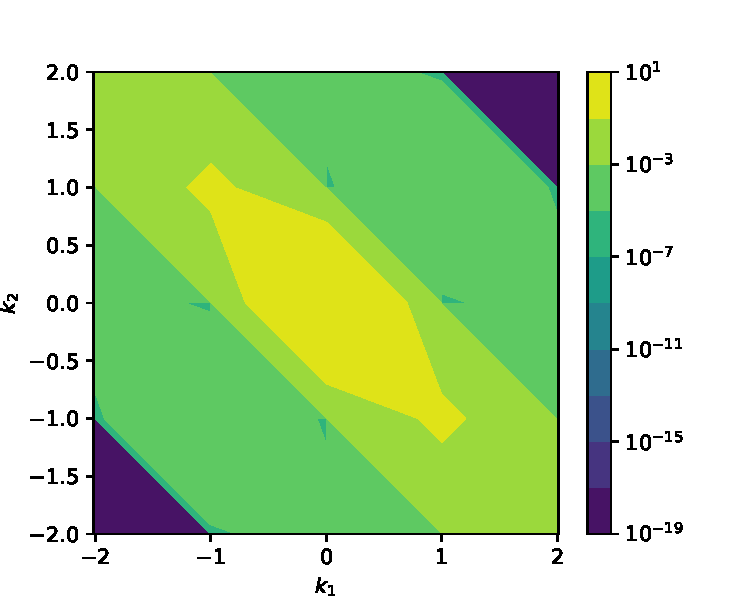
\includegraphics[width=\textwidth]{figures/2d_fourier_self_convergence_state_2.pdf}
    \caption{$k_\text{max} = 2$}
  \end{subfigure}
  ~
  \begin{subfigure}{0.48\textwidth}
    \centering
    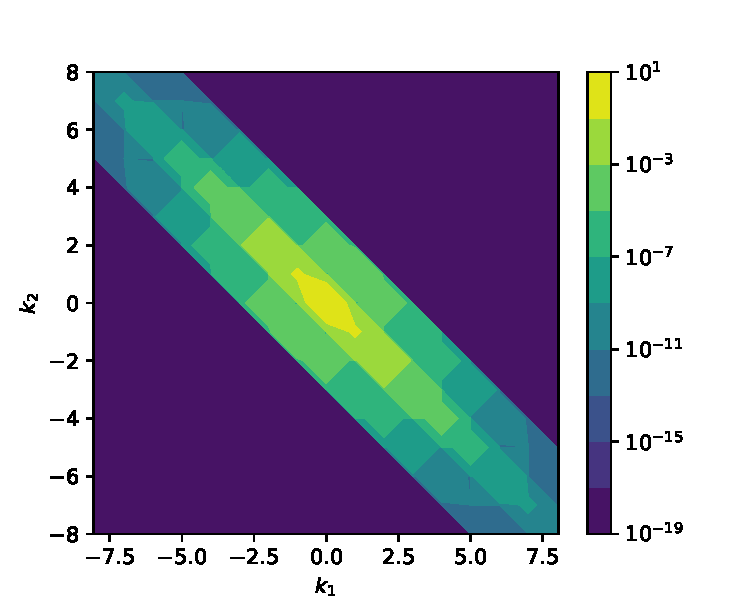
\includegraphics[width=\textwidth]{figures/2d_fourier_self_convergence_state_8.pdf}
    \caption{$k_\text{max} = 8$}
  \end{subfigure}
  \caption{The computed eigenstate corresponding to minimal energy at two
  spectral discertization levels using the Fourier scheme. We can clearly see
  that the high-energy modes are concentrated within the low-frequency regime.}
  \label{fig:2d-fourier-self-convergence-solution}
\end{figure}

\begin{figure}
  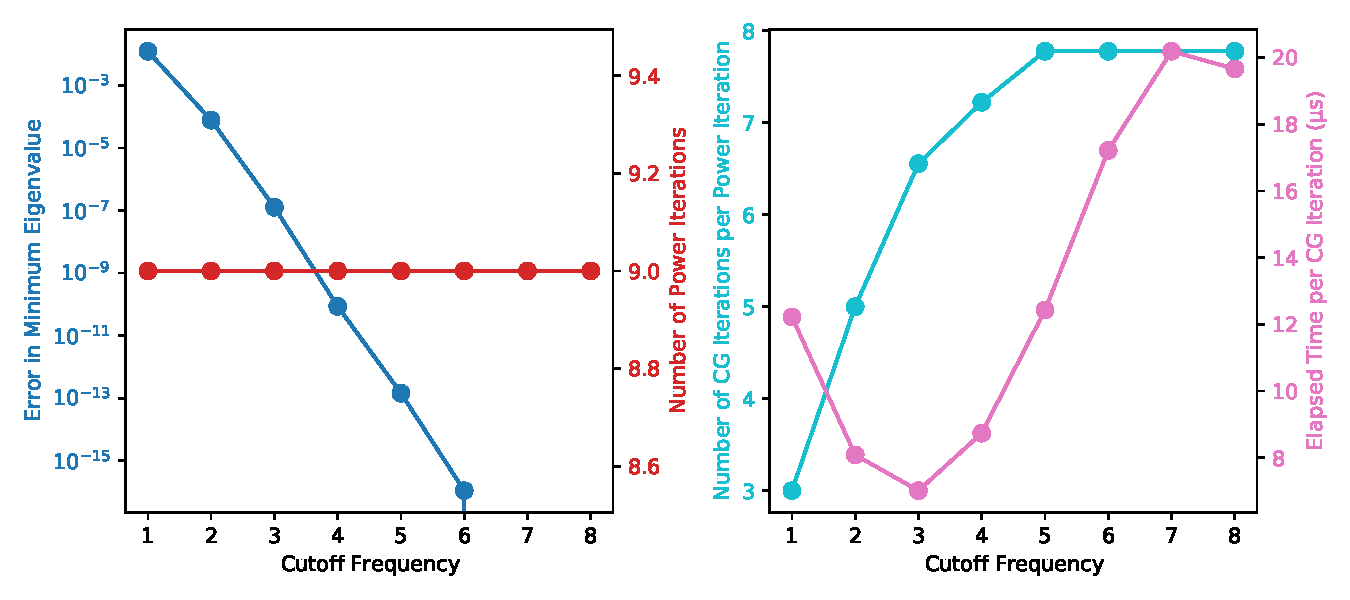
\includegraphics[width=\textwidth]{figures/2d_fourier_self_convergence_analysis.pdf}
  \caption{Performance of the Fourier scheme with quantum rotor network $\CV =
  \{1, 2\}$ and $\CE = \{(1, 2)\}$ as we increase the cutoff frequency
  $k_\text{max}$. The error in minimal eigenvalue estimates were computed using
  the $k_\text{max} = 8$ solution as reference. In our experiment, there was no
  difference in eigenvalue estimates using $k_\text{max} = 7$ and $k_\text{max}
  = 8$. The error plot clearly shows spectral convergence of the Fourier
  scheme. Also note that the average number of CG iterations per power
  iterations plateaus very quickly.}
  \label{fig:2d-fourier-self-convergence-analysis}
\end{figure}

\begin{figure}
  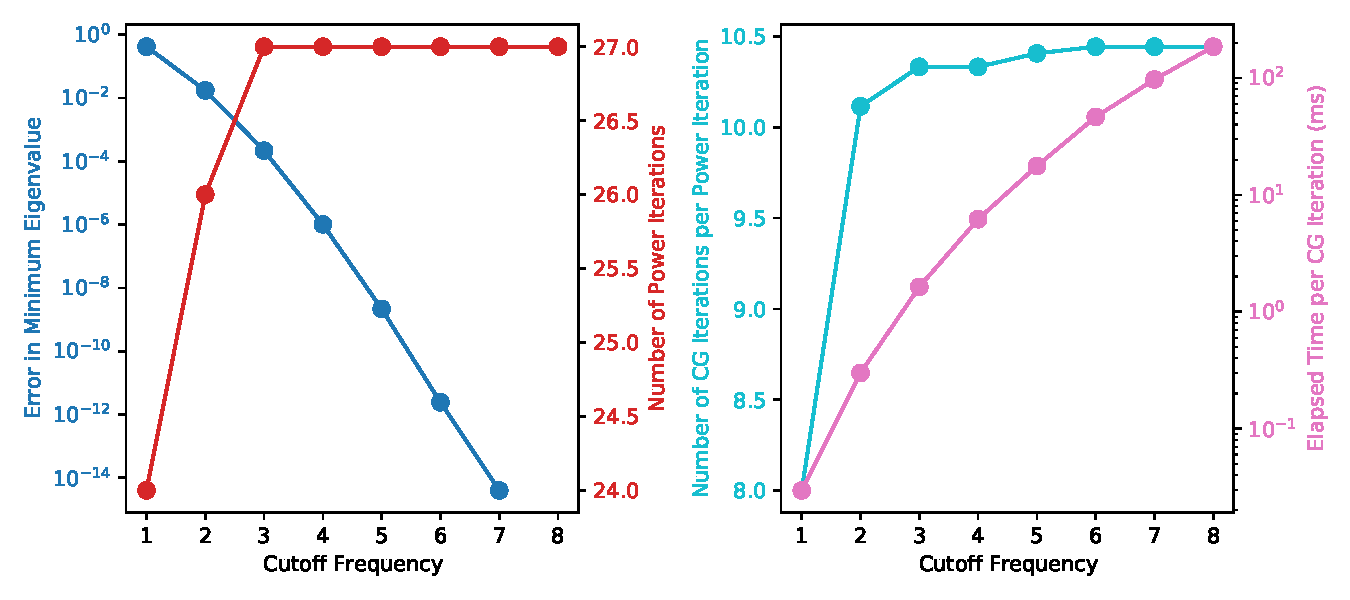
\includegraphics[width=\textwidth]{figures/5d_fourier_self_convergence_analysis.pdf}
  \caption{Performance of the Fourier scheme in a star-shaped quantum rotor
  network with $\CV = \{1, 2, 3, 4, 5\}$ and $\CE = \{(1, 3), (2, 4), (3, 5),
  (4, 1), (5, 2)\}$ as we increase the cutoff frequency $k_\text{max}$. The
  error in minimal eigenvalue estimates were computed using the $k_\text{max} =
  8$ solution as reference. The error plot clearly shows spectral convergence
  of the Fourier scheme. Also note that the average number of CG iterations per
  power iterations plateaus very quickly.}
  \label{fig:5d-fourier-self-convergence-analysis}
\end{figure}

We performed a self-convergence analysis using this Fourier scheme with exactly
the same setting as before. In implementing the CG iterations, we used the
preconditioner
\begin{equation}
  M_\mu \hat{\psi}(\Vec{k}) := \frac{g J}{2} \Norm{\Vec{k}}^2 \hat{\psi}(\Vec{k}) - \mu \hat{\psi}(\Vec{k})
\end{equation}
in solving linear system $(\hat{H} - \mu I) \widetilde{\psi}^{(\ell + 1)} =
\hat{\psi}^{(\ell)}$. In Figure~\ref{fig:2d-fourier-self-convergence-solution}
we can clearly see that the high-amplitude modes are contained within the
low-frequency domain. This leads to spectral convergence of our scheme, as
demonstrated in Figures~\ref{fig:2d-fourier-self-convergence-analysis}
and~\ref{fig:5d-fourier-self-convergence-analysis}. This leads to very few
conjugate gradient steps (all the linear solves converged within 8 iterations).
In the same figure we plot the total number of CG iterations and elapsed time
till convergence as we increase the discretization parameter $k_\text{max}$ ---
we see that the number of iterations plateaus very quickly.

\subsection{Performance of the Fourier Scheme}

\begin{figure}
  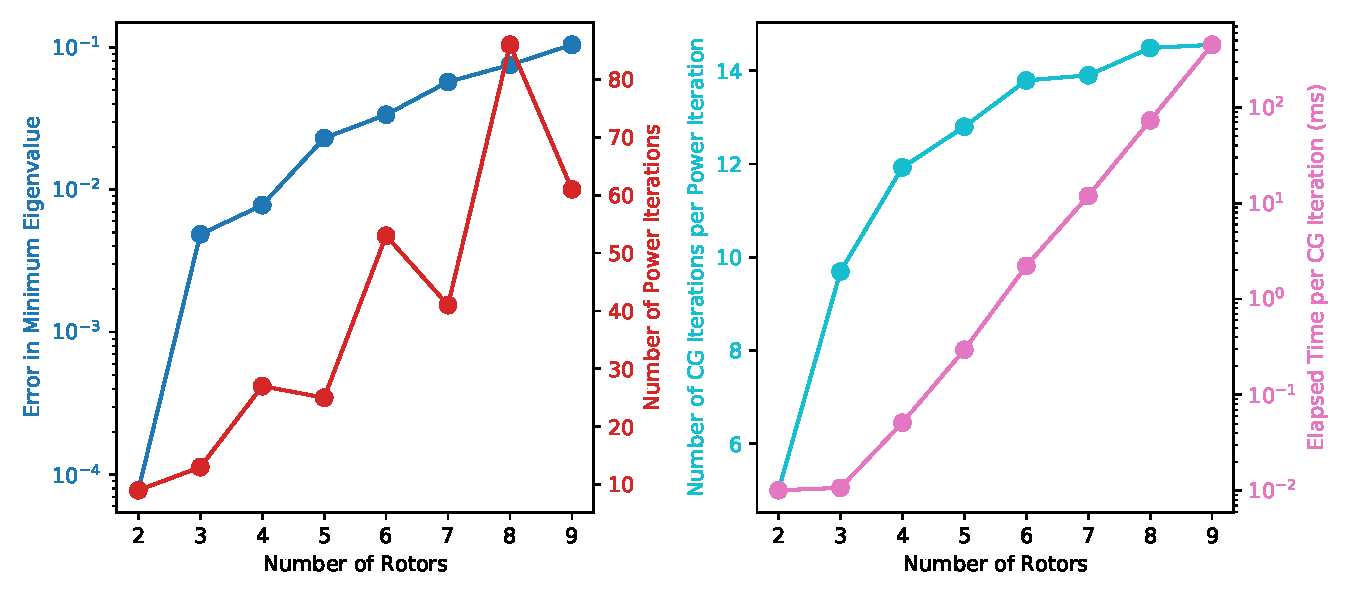
\includegraphics[width=\textwidth]{figures/2d_fourier_performance_analysis.pdf}
  \caption{Error in minimal eigenvalue, number of power iterations till
  convergence, number of CG iterations per power iteration and elapsed time per
  CG iteration with $\CV = \{1, \ldots, d\}$ and $\CE = \{(1, 2), (1, 3),
  \ldots, (1, d)\}$ as we increase the number of rotors $d$. All simulations
  were conducted with $k_\text{max} = 2$, and the error in minimum eigenvalue
  was computed with the solution with $k_\text{max} = 3$ as the reference
  solution.}
  \label{fig:2d-fourier-performance-analysis}
\end{figure}

We also tested the performance of the periodic scheme by solving the problem
for increasing number of rotors $d$. We used $k_\text{max} = 2$ for our
simulations, and used the $k_\text{max} = 3$ solution as the reference to
compute the error. In all simulations, the edge sets were set to
\begin{equation}
  \CE = \{(1, 2), (1, 3), \ldots, (1, d)\}
\end{equation}
In Figure~\ref{fig:2d-fourier-performance-analysis} we plot the error in the
minimal eigenvalue, number of power iterations, number of CG iterations per
power iteration and elapsed time per CG iteration.

\subsection{Parallel Performance}

\begin{figure}
  \centering
  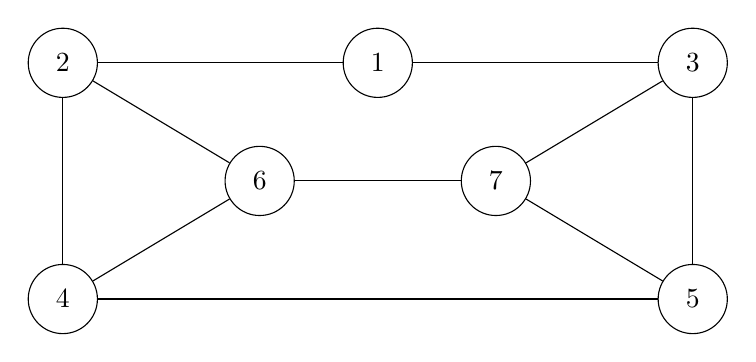
\begin{tikzpicture}
    \node[state] (A) at ( 0, 3) {1};
    \node[state] (B) at (-4, 3) {2};
    \node[state] (C) at ( 4, 3) {3};
    \node[state] (D) at (-4, 0) {4};
    \node[state] (E) at ( 4, 0) {5};
    \node[state] (F) at (-1.5, 1.5) {6};
    \node[state] (G) at ( 1.5, 1.5) {7};

    \draw (A) -- (B);
    \draw (A) -- (C);
    \draw (B) -- (D);
    \draw (C) -- (E);
    \draw (B) -- (F);
    \draw (C) -- (G);
    \draw (D) -- (F);
    \draw (E) -- (G);
    \draw (D) -- (E);
    \draw (F) -- (G);
  \end{tikzpicture}
  \caption{Quantum rotor network used in simulation to determine parallel
  performance of our OpenMP based parallel Fourier scheme.}
  \label{fig:quantum-rotor-network}
\end{figure}

We note that our algorithm is easily parallelizable, both with the basic and
Fourier schemes, and using either distributed or shared memory frameworks. We
implemented a basic parallel code utilizing OpenMP. In this framework, we
solved a problem with $d = 7$ quantum rotors and discretization level
$k_\text{max} = 8$ using the Fourier scheme. The edges between the rotors were
distributed as in Figure~\ref{fig:quantum-rotor-network}. In
Table~\ref{tab:strong-scaling} we present the results from the strong scaling.

\begin{table}
  \renewcommand*{\arraystretch}{1.3}
  \centering
  \begin{tabular}{c | c | c}
    \hline
    OpenMP Threads & Elapsed Time (hrs) & Speed-up\\
    \hline
    1 & 45.6 &  --  \\
    2 & 28.6 & 1.59 \\
    4 & 23.7 & 1.92 \\
    8 & 16.1 & 2.83 \\
    \hline
  \end{tabular}
  \vspace{1em}
  \caption{Strong scalability of the OpenMP based parallel Fourier scheme with
  quantum rotor network as defined in Figure~\ref{fig:quantum-rotor-network}
  with $k_\text{max} = 8$.}
  \label{tab:strong-scaling}
\end{table}

\subsection{Comparison with VMC Solver}

We now compare our PDE based solver against the VMC solver. In this set of
experiments, we use a simple chain as the quantum rotor network.

\begin{table}
  \renewcommand*{\arraystretch}{1.3}
  \centering
  \begin{tabular}{c | r r | r r | r r}
    \hline
        & \multicolumn{2}{c|}{PDE ($k_\text{max} = 5$)}
        & \multicolumn{2}{c|}{PDE ($k_\text{max} = 7$)}
        & \multicolumn{2}{c}{VMC} \\
    \cline{2-7}
    $d$ & $\lambda_\text{min}$ & $T_\text{elapsed}$ & $\lambda_\text{min}$
        & $T_\text{elapsed}$ & $\lambda_\text{min}$ & $T_\text{elapsed}$ \\
    \hline
    2 & $-0.075$ &  $0.090$ & $-0.075$ &   $0.093$ & $-0.076$ & $35$ \\
    3 & $-0.153$ &  $0.216$ & $-0.153$ &   $0.169$ & $-0.154$ & $40$ \\
    4 & $-0.231$ &  $0.523$ & $-0.231$ &   $0.692$ & $-0.239$ & $45$ \\
    5 & $-0.310$ &  $2.262$ & $-0.310$ &   $7.896$ & $-0.306$ & $63$ \\
    6 & $-0.388$ & $27.359$ & $-0.388$ & $337.720$ & $-0.384$ & $98$ \\
    \hline
  \end{tabular}
  \vspace{1em}
  \caption{Comparison of the PDE and HMC based solvers on a quantum rotor
  network consisting of $d$ sites on a chain. We record the minimal eigenvalue
  and elapsed time (in seconds).}
  \label{tab:pde-hmc}
\end{table}

\end{document}
